\chapter{Variational Auto-encoders and Generative Adversarial Networks}

\section{Variational Auto-Encoders}
% Authors: Yu Cao, Evgenii Nikitin, Aishwarya Budhkar (editor), 4/16/2019
% Editor: Benjamin Ahlbrand
\begin{figure}[H]
    \centering
    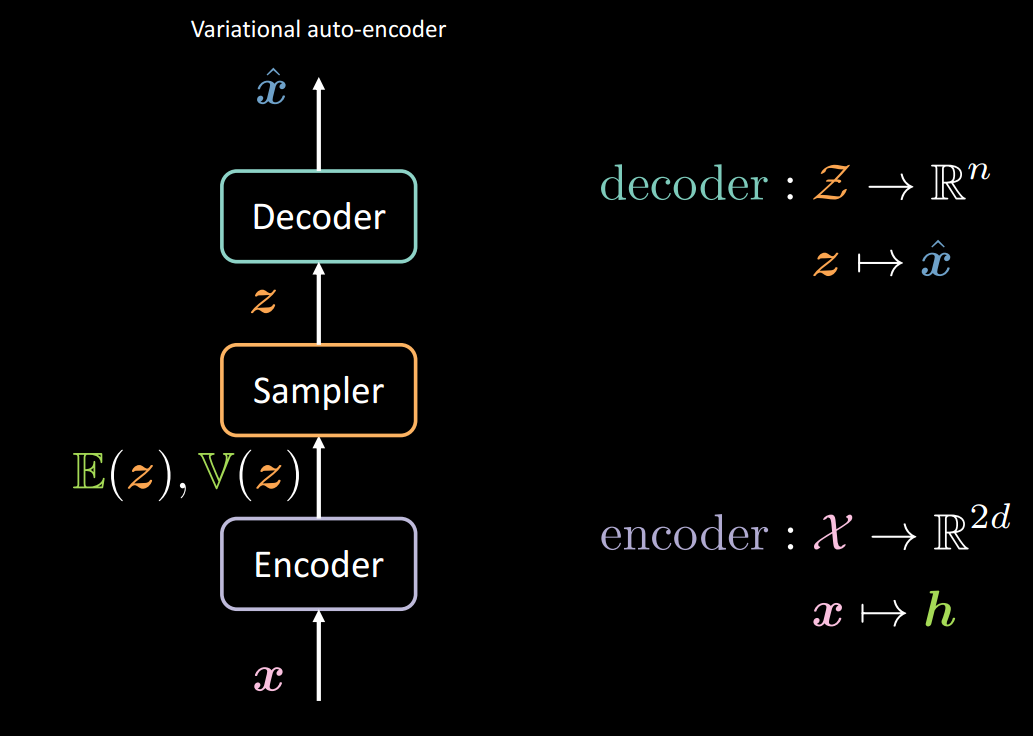
\includegraphics[width=0.7\textwidth]{figs/vae.png}
    \caption{Architecture of Variational Autoencoder}
    \label{fig:vae}
\end{figure}

There are two types of basic autoencoders: over-complete and under-complete. A type of constraint which can be applied is information bottlenecking - this is a reduction in the size of intermediate layer which results in an under-complete autoencoder. In over-complete autoencoders there is larger intermediate layer so we can extract better meaningful features. Variational AutoEncoders (VAE) inherit the architecture of the traditional autoencoders described previously. However, there is a key difference between them -- in contrast to the encoder in a vanilla autoencoder outputting a hidden representation $h$ of the input $x$, the VAE encoder produces two vectors -- expectation $E(z)$ and variance $V(z)$ over latent variable $z$ (Figure \ref{fig:vae}). This property allows us to produce stochastic representations of the input. This is achieved by sampling a vector from a gaussian distribution with zero mean and unit variance and shifting and rescaling vector elements according to estimated $E(z)$ and $V(z)$ respectively:
\begin{align*}
    \vect{z'} &= \mathop{\mathbb{E}}(\vect{z}) + \vect{\epsilon} \odot \sqrt{\mathop{\mathbb{V}}(\vect{z})} \\
    \vect{\epsilon} &\sim \mathcal{N}(0, \mathcal{I}_d)
\end{align*}

After that, sampled representation $z'$ is decoded into output $\hat{x}$. In order to make sure that this output is close to the input $x$, we introduce a reconstruction component of the loss function -- $\ell(x,\hat{x})$ (e.g., mean-squared error loss or binary cross-entropy depending on the nature of the data).

\begin{figure}[H]
    \centering
    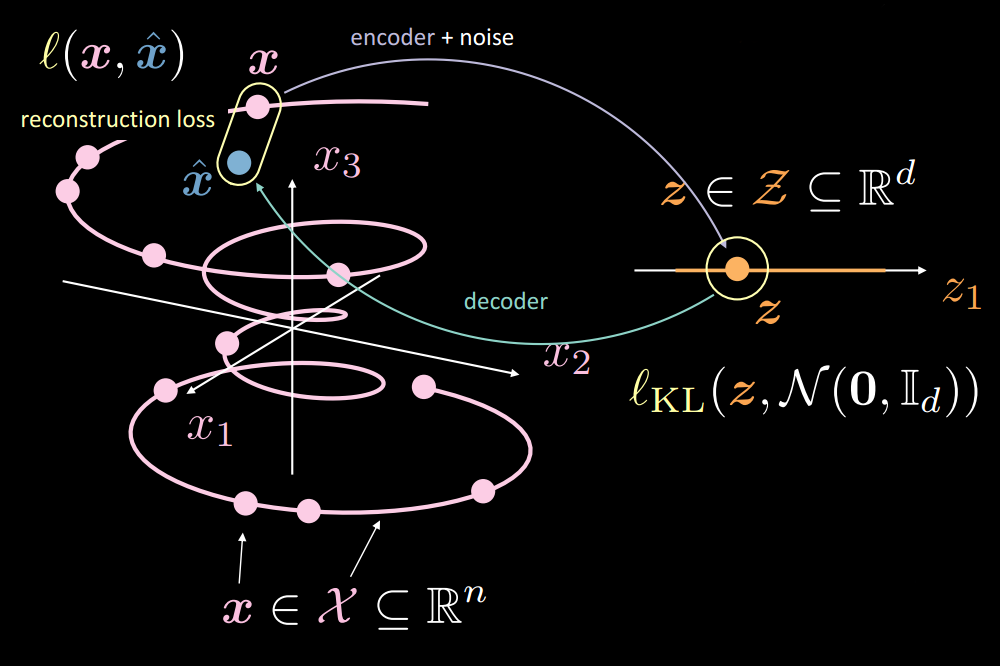
\includegraphics[width=0.7\textwidth]{figs/vae_expl.png}
    \caption{Visualization of encoding and decoding processes}
    \label{fig:vae_expl}
\end{figure}

However, as there is no limit on the values of $E(z)$ and $V(z)$, the encoder can learn to push different training samples very far apart in the latent space (Figure \ref{fig:bubbles_rec}), effectively reconstructing the training data. In order to avoid this, we introduce a constraint by adding KL-divergence component to the loss function.
\begin{align*}
    \ell(x, \hat{x}) = \ell_{rec} + \beta \ell_{KL} (z, \mathcal{N}(0, \mathcal{I}_d)) \simeq \ell_{rec} + \beta\sum_{i=1}^d (\mathop{\mathbb{V}}(\vect{z}) - \log{\mathop{\mathbb{V}}(\vect{z})} - 1 + \mathop{\mathbb{E}}(\vect{z})^2)_i
\end{align*}

Intuitively, this new term forces learned representations of the training samples to have unit variance and to be as close to zero as possible (Figure \ref{fig:bubbles_kl}). $\beta$ is a hyperparameter that controls the tightness of the constraint. Reconstruction loss ensures that the different "bubbles" do not overlap, the network still reconstructs the different inputs, while adding KL-divergence to the reconstruction loss seeks to confine them to the most compact space possible. This feature of VAEs leads to a smooth learned latent spaces, allowing interpolation between the different samples and / or classes continuously.

\begin{figure}[H]
    \centering
    \begin{subfigure}[b]{.45\linewidth}
    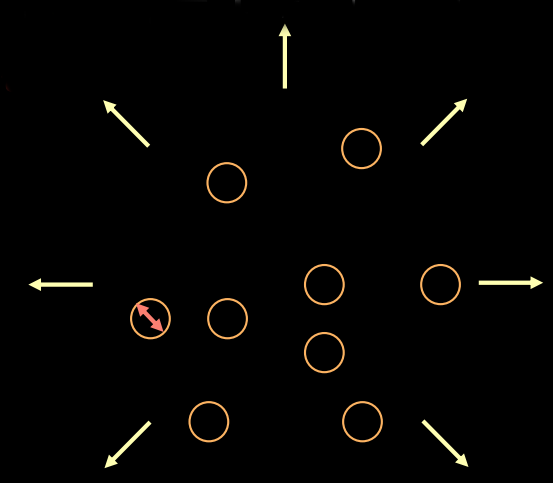
\includegraphics[width=\linewidth]{figs/bubbles_rec.png}
    \caption{Samples get pulled apart by reconstruction loss}\label{fig:bubbles_rec}
    \end{subfigure}
    \begin{subfigure}[b]{.45\linewidth}
    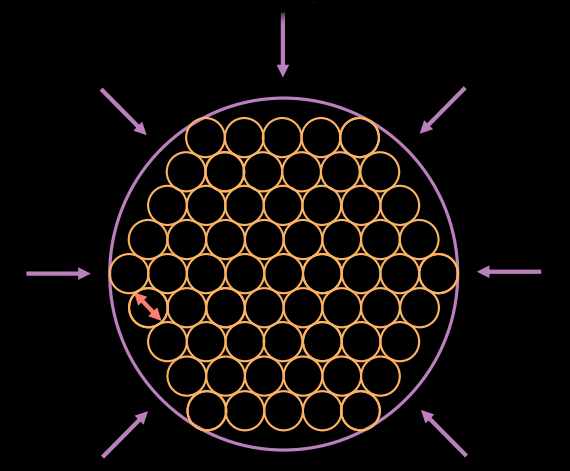
\includegraphics[width=\linewidth]{figs/bubbles_kl.png}
    \caption{Samples get pushed towards zero by KL-divergence loss}\label{fig:bubbles_kl}
    \end{subfigure}
    \caption{Effects of the different loss components}
    \label{fig:bubbles}
\end{figure}

\section{Generative Adversarial Network}
\subsection{Introduction}
\begin{figure}
    \centering
    \includegraphics[width=0.7\textwidth]{"figs/VAE and GAN".png}
    \caption{Architecture of GAN}
    \label{fig:gan_arch}
\end{figure}

As shown in the above figure. The GAN model is conceptually similar to the VAE model.

Consider a money counterfeiter. The $\hat{x}$ produced by sampler+generator can be thought as the fake money he makes. He then tries to deposit the money at a bank (the discriminator), who obviously wants to differentiate fake money from the genuine article ($x$). If the fake money is not 'convincing' enough, the discriminator will provide feedback, stating such, (through back-propagation) and the counterfeiter can improve his skills (gradient descent), until the discriminator can not tell the fake one apart from the genuine one.

Using the sampler we generate noise. On top of the sampler we have the generator which attempts to produce authentic data, similar to the decoder in auto-encoders -- both of which are generative networks. From the generator we get our estimate $\hat{x}$ on the manifold. The estimate, together with our real $x$, is sent to a discriminator which distinguishes $x$ from $\hat{x}$ that is difference between fake and actual values. We can optimize the generator based on what fools and does not fool the discriminator

The generator maps the latent space to input space $\begin{array}{r}{G : \mathcal{Z} \rightarrow \mathbb{R}^{n}}, {z \mapsto \hat{x}}\end{array}$

Whereas the discriminator, we go from the original input ($x$) or the generated input ($\hat{x}$) to a learned loss. $\begin{aligned} D : & \mathbb{R}^{n} \rightarrow(0,1) & x \vee \hat{x} \mapsto \ell \end{aligned}$

\subsection{Model illustration}

\begin{figure}
    \centering
    \includegraphics[width=0.7\textwidth]{"figs/GAN illustration".png}
    \caption{Visualization of encoding and decoding process}
    \label{fig:enc_dec_process}
\end{figure}

We start from a random variable in the hidden space. Then $\hat{x}$ is sampled from the generator. Note that in the GAN setting, we do not know our data manifold, so unlike using reconstruction to approximate $\hat{x}$ to data manifold. We apply our discriminator on both the generated data and real data. We train our discriminator so that it can tell apart the two. On the other hand, we get the gradient, so that we can make the generated data as close to the real data manifold as possible. \\

When training GANs, we don't use a traditional loss function as the scheme here is that of a min-max game. Hence, we instead perform an adversarial loss. See the following equation:

$$V(D, G)=\mathbb{E}_{\boldsymbol{x} \sim p_{\text { data }}(\boldsymbol{x})}[\log D(\boldsymbol{x})]+\mathbb{E}_{\boldsymbol{z} \sim p_{\boldsymbol{z}}(\boldsymbol{z})}[\log (1-D[G(\boldsymbol{z})])]$$
$$\min _{G} \max _{D} V(D, G)$$

The above function achieves a Nash equilibrium between the performance of the discriminator and the performance of the generator. When the two modules converge together, the discriminator should determine fake versus real data, and the generator would generate perfect data.